%--------------------------------------
%ELECTROTECHNIQUE - SCHEMA DE LIAISON A LA TERRE
%--------------------------------------

%utiliser les environnement \begin{comment} \end{comment} pour mettre en commentaire le préambule une fois la programmation appelée dans le document maître (!ne pas oublier de mettre en commentaire \end{document}!)

%\begin{comment}

\documentclass[a4paper, 11pt, twoside, fleqn]{memoir}

\usepackage{AOCDTF}

\marqueurchapitre

%lien d'édition des figures Tikz sur le site mathcha.io (rajouter le lien d'une modification effectuée sur la figure tikz avec le nom du modificateur car il n'y a qu'un lien par compte)

%lien mathcha Nom Prénom : 

%--------------------------------------
%corps du document
%--------------------------------------

\begin{document} %corps du document
	\openleft %début de chapitre à gauche

%\end{comment}

\begin{landscape}

\begin{xltabular}{\textwidth}{c X X X c}
\caption{Déclinaisons du SLT TN}\\
\toprule
\thead{Nom}		& \thead{Caractéristiques}		& \thead{Avantages}		& \thead{Inconvénients} & \thead{Schéma sain} \\
\midrule
\endfirsthead %en-tête de la première page du tableau  
\multicolumn{5}{l}{\small\textit{Page précédente}} \\
\midrule %filet de milieu de tableau
\thead{Nom}		& \thead{Caractéristique}		& \thead{Schémas} 	& \thead{Inconvénients} 	& \thead{Schéma sain} \\
\midrule
\endhead
\midrule %filet de milieu de tableau
\multicolumn{5}{r}{\small\textit{Page suivante}} \\
\endfoot %pied de page de toutes les pages du tableau
\bottomrule
\endlastfoot %pied de page de la dernièredu tableau
Confondus (TN-C)		
& 
\begin{tabitemize}
\item Conducteurs neutre et PE confondus\,;
\item PE et neutre vert/jaune nommé conducteur Protection \'Equipotentielle Neutre (PEN)\,;
\item Connexion à la \emph{prise de terre du neutre} du poste HT/BT.
\end{tabitemize}
&
\begin{tabitemize}
\item économie d'un câble.
\end{tabitemize}
&		
\begin{tabitemize}
\item utilisation de canalisations fixes et rigides\,;
\item interdiction de pose :
	\begin{tabitemize}
	\item locaux à risques d'incendies\,;
	\item alimentation d'équipements de traitement de l'information (présence de courant harmonique dans le neutre).
	\end{tabitemize}
\end{tabitemize}	
& 
\adjustbox{valign=t}{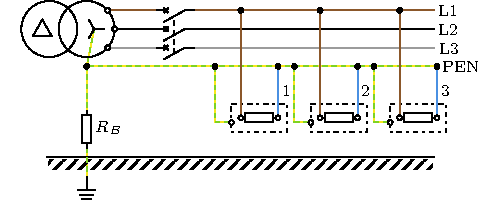
\includepdf{fig_schema_tn-c_sain.pdf}}
\\

\end{xltabular}

\end{landscape}

\end{document}

